\documentclass{standalone}
\usepackage{../mss}
\usepackage{sansmath}
\usepackage{tikz}
\usetikzlibrary{shapes.geometric,positioning,calc,petri,graphs,fit,backgrounds}
\tikzset{
        node distance=0.2cm and 2.0cm,
        >=latex,
        font=\sf\bfseries\sansmath,
        textfeld/.style={align=center,minimum height=1cm,minimum width=1.5cm},
        pfeil/.style={->,line width=1.1pt},
        box/.style={rectangle,draw,line width=1.1pt,minimum height=1.5cm,minimum width=2.8cm,align=center},
        segment/.style={rectangle,draw,dashed,rounded corners=3mm,minimum height=1.5cm,minimum width=2.8cm},
        generator/.style={rectangle,draw,fill=gray!5,dashed,rounded corners=3mm,minimum height=1cm,minimum width=1cm}
        }
\tikzgraphsset{
    every graph/.style = {use existing nodes}
}
\begin{document}

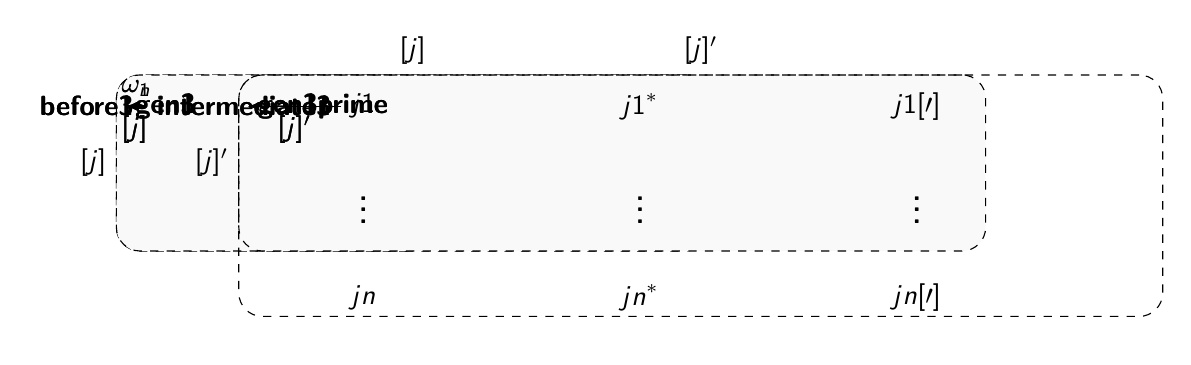
\begin{tikzpicture}

        \node[textfeld] (before1) {};
        \node[textfeld] (before2)[below= of before1] {};
        \node[textfeld] (before3)[below= of before2] {};

        \node[textfeld] (gen1) [right= of before1]{$ \localmarking{j1} $};
        \node[textfeld] (gen2) [below= of gen1]{$ \vdots $};
        \node[textfeld] (gen3) [below= of gen2]{$ \localmarking{jn} $};

        \node[textfeld] (intermediate1) [right= of gen1]{$ \localmarking{j1}^* $};
        \node[textfeld] (intermediate2) [right= of gen2]{$ \vdots $};
        \node[textfeld] (intermediate3) [right= of gen3]{$ \localmarking{jn}^* $};

        \node[textfeld] (gen1prime) [right= of intermediate1]{$ \localmarking{j1}[\prime] $};
        \node[textfeld] (gen2prime) [right= of intermediate2]{$ \vdots $};
        \node[textfeld] (gen3prime) [right= of intermediate3]{$ \localmarking{jn}[\prime] $};
        \node[right=of gen3prime](anonymous)  {};
        \graph{
        before1 ->[edge label={$ \synchronization[j] $}]gen1 ->[edge label={$ \omega_1 $}] intermediate1 ->[edge label={$ \synchronization[j]^\prime $}] gen1prime
        };
        \graph{
        before3 ->[edge label={$ \synchronization[j] $}]gen3 ->[edge label={$ \omega_n $}] intermediate3 ->[edge label={$ \synchronization[j]^\prime $}] gen3prime
        };
        \begin{scope}[on background layer]
                \node[segment, fit=(gen1)(intermediate1)(gen2)(intermediate2)(gen3)(intermediate3), label={above:$ \segment[j] $}] (o) {};
                \node[generator, fit=(gen1)(gen2)(gen3), label={left:$ \generator[j] $}] (o) {};
                \node[generator, fit=(gen1prime)(gen2prime)(gen3prime), label={left:$ \generator[j]^\prime $}] (o) {};
                \node[segment, fit=(gen1prime)(gen2prime)(gen3prime)(anonymous), label={above:$ \segment[j]^\prime $}] (o) {};
        \end{scope}

\end{tikzpicture}
\end{document}